\section{Corrected Synthetic Diagnostics}

All evidence in this section comes from the corrected synthetic review snapshot
accepted in PR~\#4. Those artifacts were generated under explicit provenance,
immutable run manifests, strict JSON outputs, common random numbers for the
stochastic setting, and figure-level source metadata. Legacy
\texttt{ALL\_RUNS.json}-style aggregates and old neural results are excluded.

\begin{figure}[t]
    \centering
    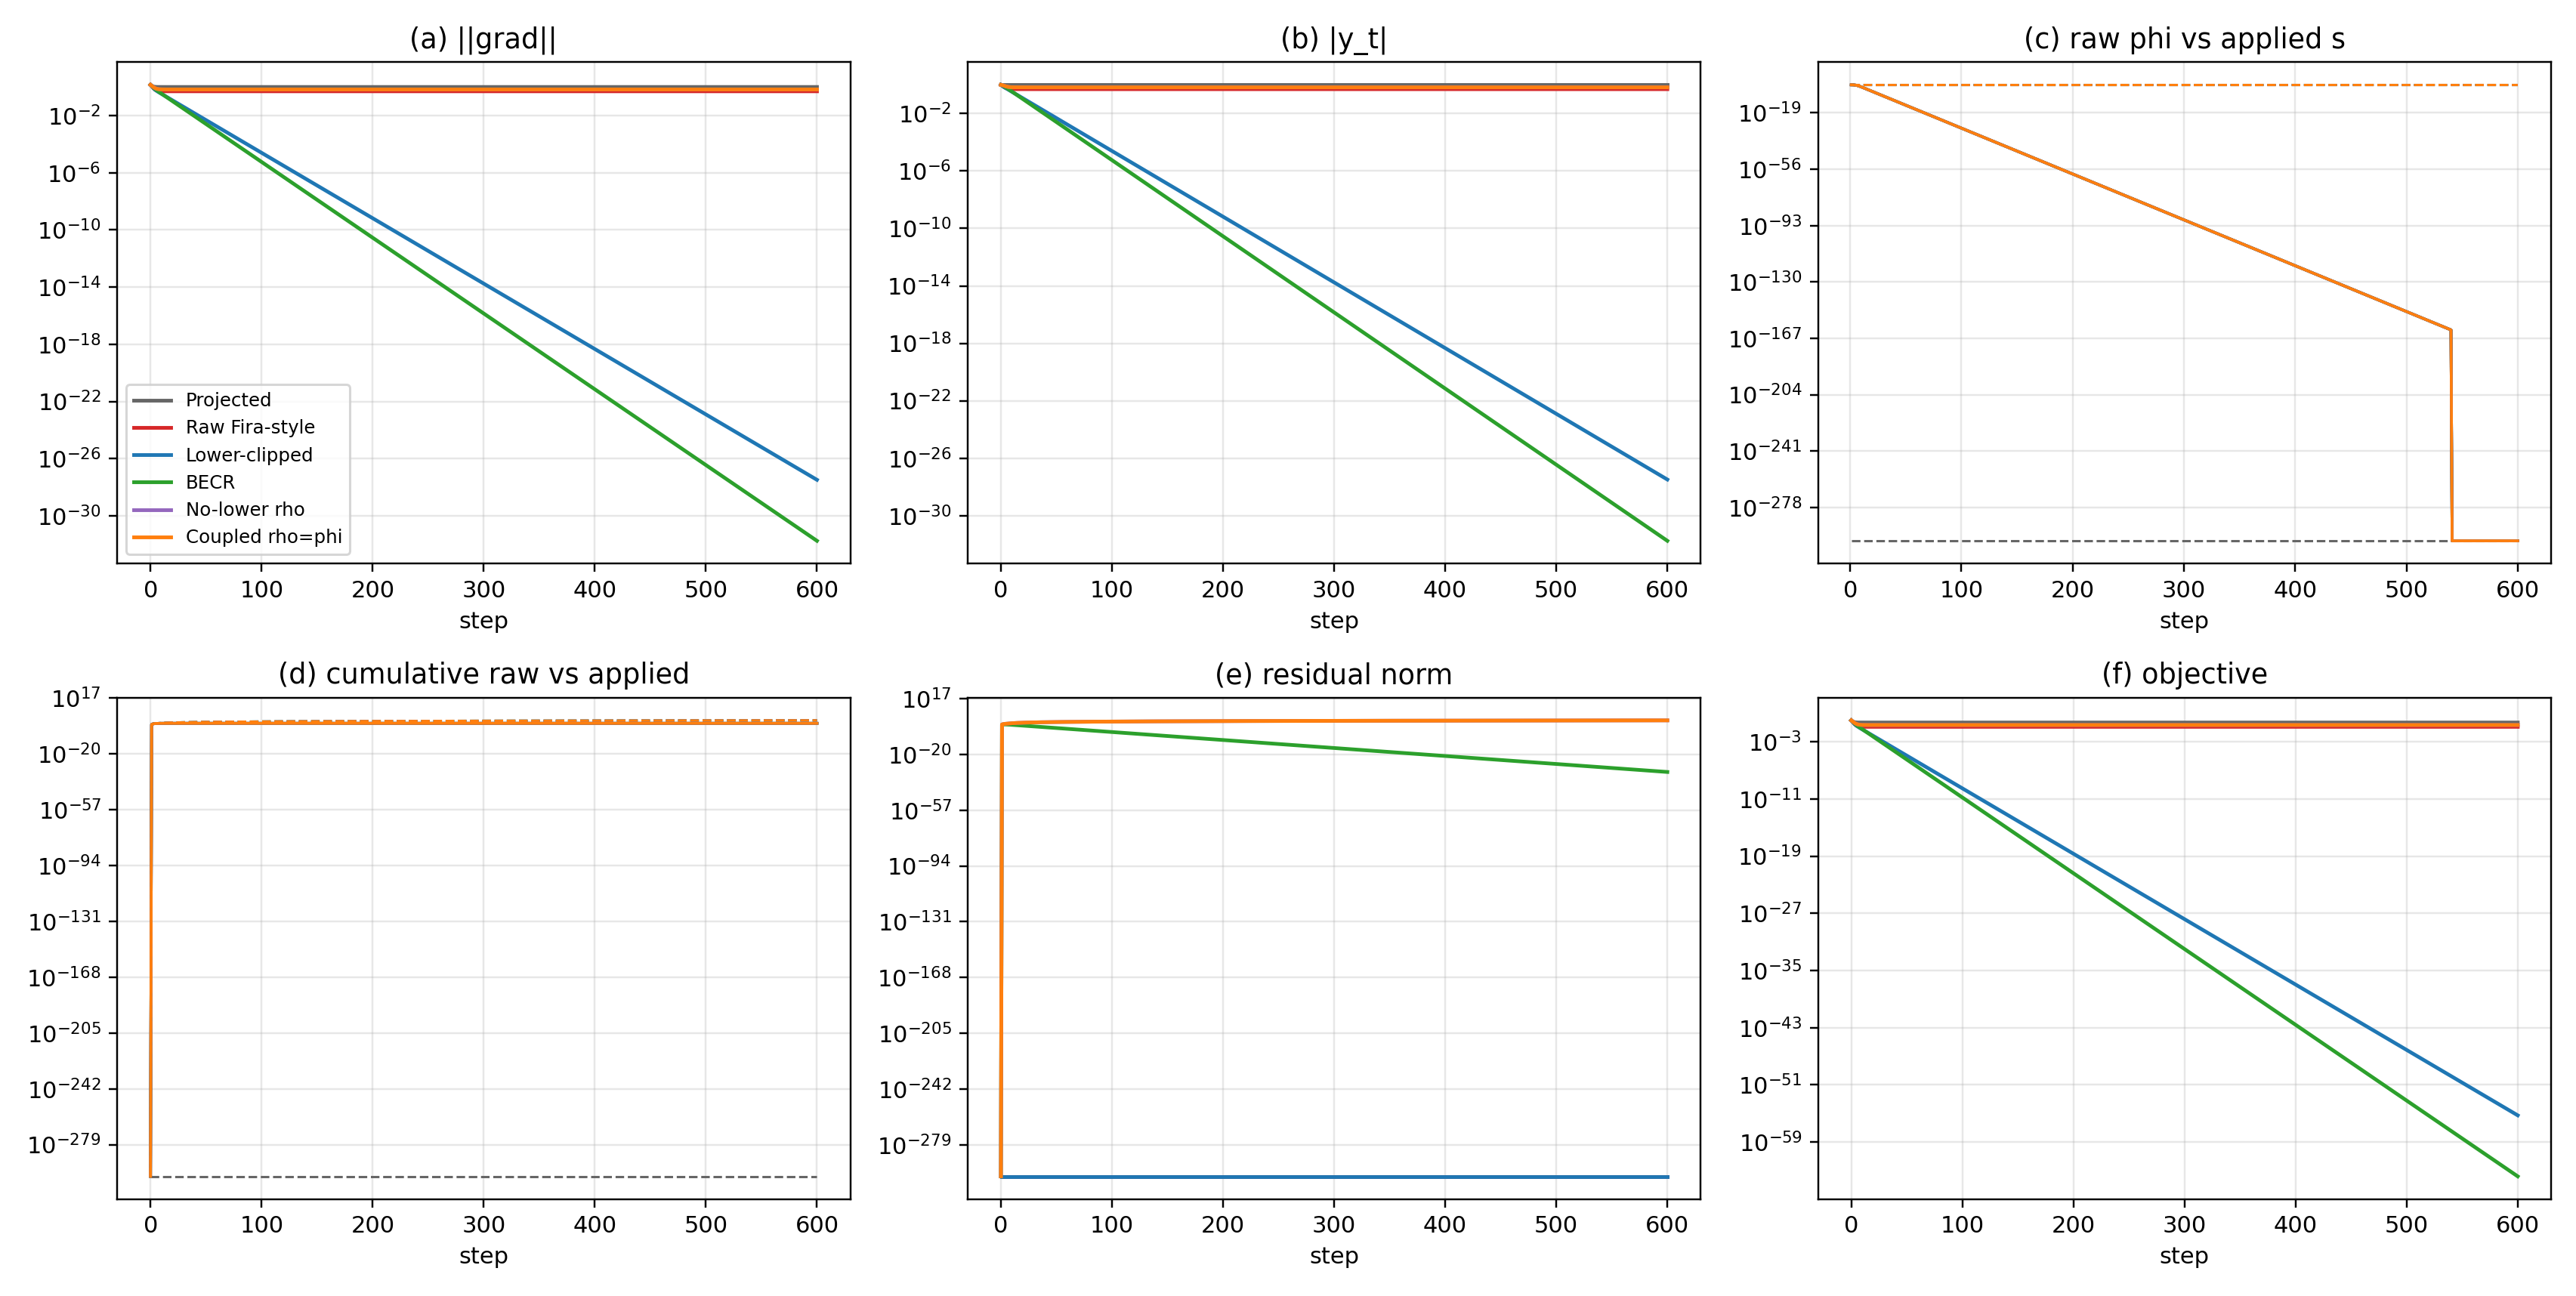
\includegraphics[width=\linewidth]{figures/figure1_theorem_regime.png}
    \caption{\textbf{Corrected theorem-regime $2$D validation.} Raw
    \Fira-style recovery drives $x_t\to 0$ but leaves a nonzero $y_t$ and
    gradient norm because the cumulative raw recovery mass plateaus.
    Lower-bounded clipping and separated $\rho/s$ \BECR\ both drive
    $\norm{\grad f}$ to zero. The no-lower-bound and coupled
    $\rho_t=\phi_t$ ablations are worse than \BECR.}
    \label{fig:theorem-regime}
\end{figure}

The theorem-regime parameters match the verified stale-subspace conditions:
$\eta a=0.5<2\epsilon_a=2.0$, $M_0=0.25$, and $\eta b M_0=0.125\le 1/2$.
Table~\ref{tab:theorem-values} records the final stationarity values used in
the accepted figure package.

\begin{table}[t]
    \caption{Verified theorem-regime values from the corrected review snapshot.}
    \label{tab:theorem-values}
    \centering
\small
\begin{tabular}{lrrrrrr}
\toprule
Method & final $x$ & final $y$ & final $\|\grad f\|$ & $\sum \phi_{\mathrm{raw}}$ & $\sum s_{\mathrm{applied}}$ & residual \\
\midrule
Projected baseline & $1.36{\times}10^{-180}$ & $1.0$ & $1.0$ & $1.318$ & $0$ & $0$ \\
Raw recovery & $1.36{\times}10^{-180}$ & $0.5$ & $0.5$ & $1.318$ & $1.318$ & $0$ \\
Clipped recovery & $1.36{\times}10^{-180}$ & $3.28{\times}10^{-28}$ & $3.28{\times}10^{-28}$ & $1.318$ & $1.20{\times}10^2$ & $0$ \\
\BECR & $1.36{\times}10^{-180}$ & $1.77{\times}10^{-32}$ & $1.77{\times}10^{-32}$ & $1.318$ & $1.20{\times}10^2$ & $2.29{\times}10^{-32}$ \\
No-lower $\rho$ & $1.36{\times}10^{-180}$ & $0.6717$ & $0.6717$ & $1.318$ & $1.20{\times}10^2$ & $4.01{\times}10^2$ \\
Coupled $\rho=\phi$ & $1.36{\times}10^{-180}$ & $0.6717$ & $0.6717$ & $1.318$ & $1.20{\times}10^2$ & $4.01{\times}10^2$ \\
\bottomrule
\end{tabular}

\end{table}

The corrected high-dimensional stale diagnostics reproduce the same mechanism
beyond $2$D. Raw recovery reduces the orthogonal gradient relative to pure
projection but still leaves a substantial stale orthogonal channel
($1.5063$ in mean norm), while clipping and \BECR\ reduce that orthogonal
channel to numerical zero. The projected branch still leaves a nonzero parallel
gradient floor ($0.2795$ mean norm), so this evidence supports only the
\emph{orthogonal stale-channel repair} claim, not universal full stationarity.

\begin{figure}[t]
    \centering
    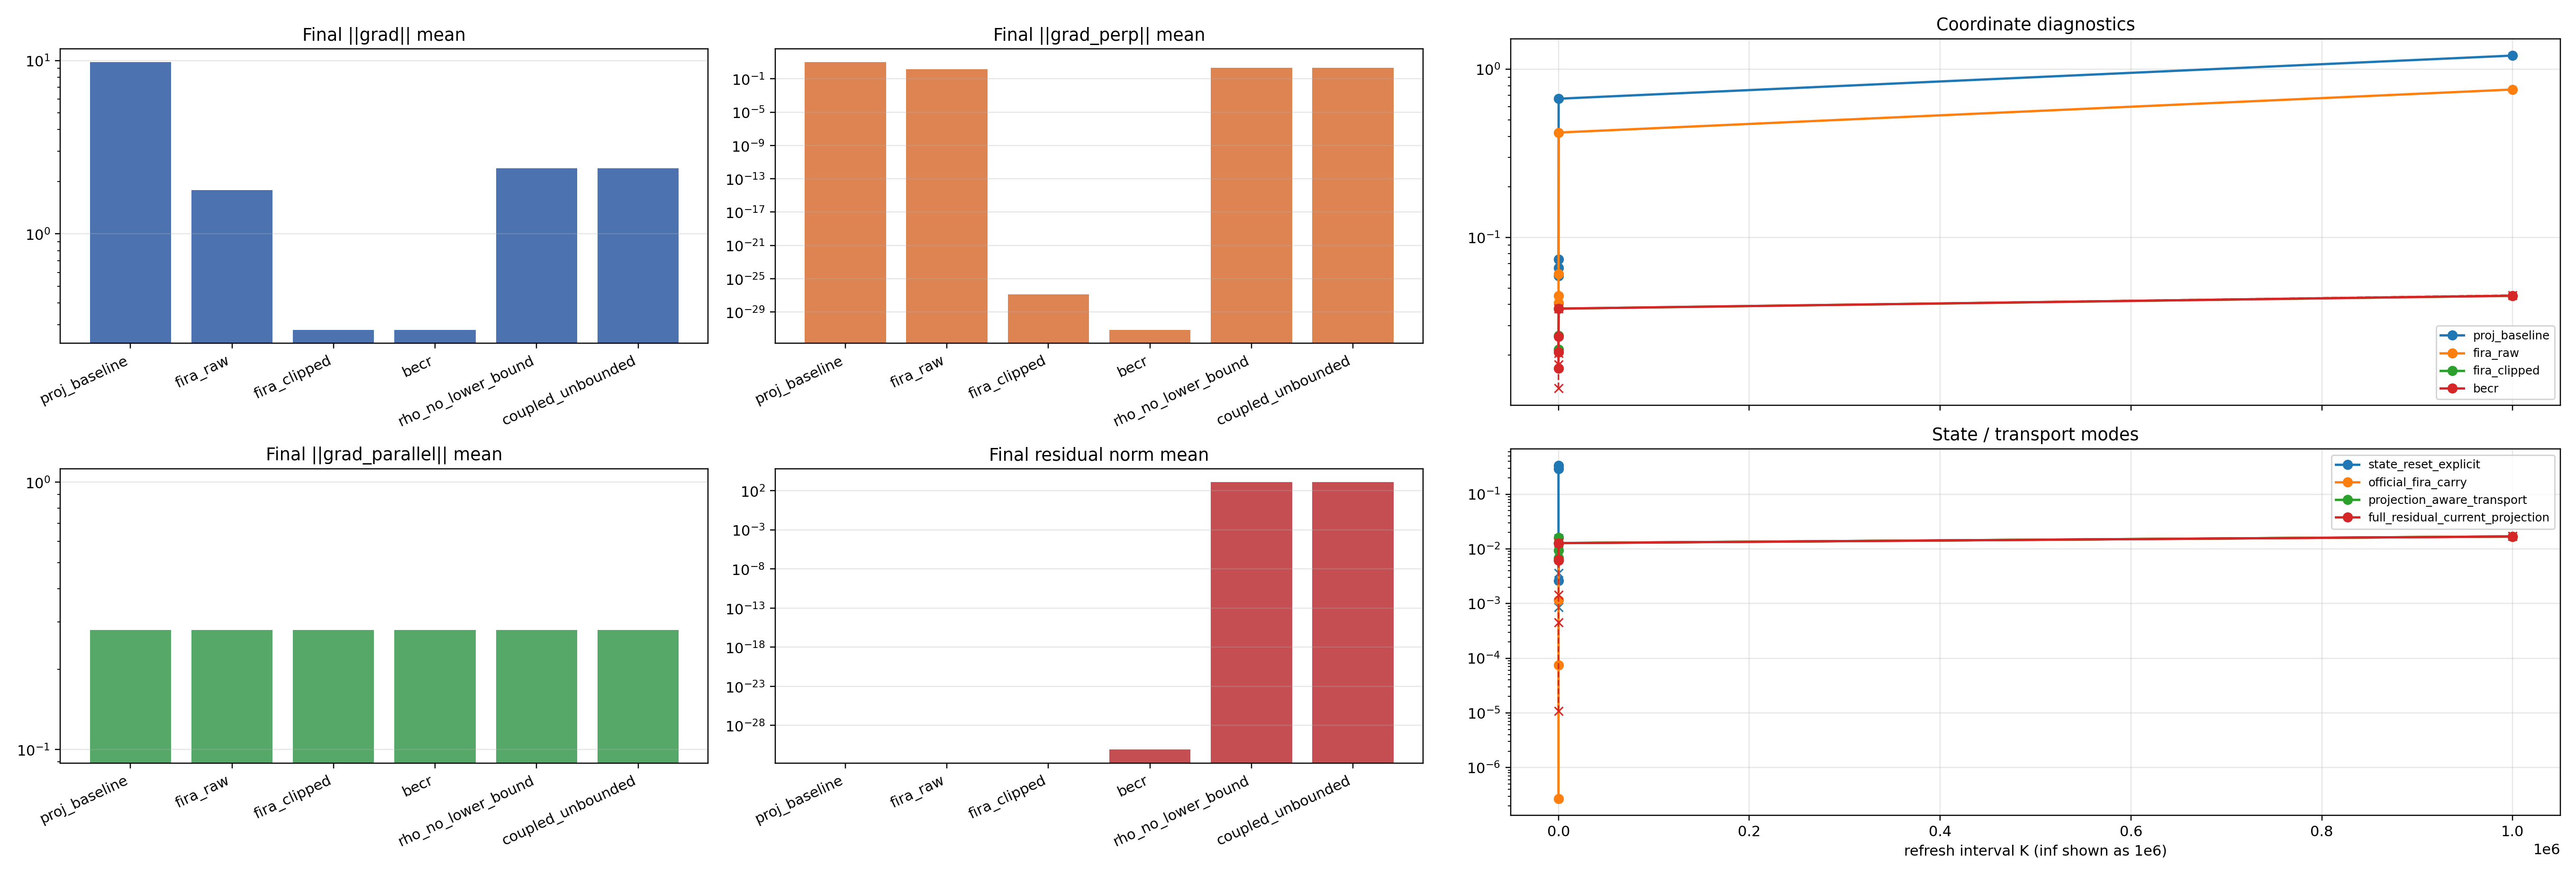
\includegraphics[width=\linewidth]{figures/figure2_highdim_refresh.png}
    \caption{\textbf{Corrected high-dimensional stale diagnostics and refresh
    sweep.} Left: fixed stale subspaces reproduce the orthogonal stale-channel
    failure beyond $2$D; clipping and \BECR\ remove the orthogonal component but
    do not remove the projected branch floor. Right: more frequent refresh
    reduces stale failure, while bounded recovery reduces sensitivity to large
    refresh gaps. This figure is a mechanism diagnostic, not an optimizer
    ranking.}
    \label{fig:highdim-refresh}
\end{figure}

The refresh sweep shows the boundary condition directly. For the coordinate
family, the final gradient norm of raw recovery grows from roughly $0.045$ at
$K=1$ to $0.759$ at $K=\infty$, whereas clipped recovery grows from $0.021$ to
$0.045$ and \BECR\ from $0.017$ to $0.045$. The state-mode traces show that
reset, official-carry, projection-aware transport, and full current-projection
residual handling lead to measurably different behavior when the subspace
changes.

The anisotropic noisy projection diagnostic is retained as a stochastic
appendix figure. In the accepted five-seed CRN setting, \BECR\ achieved mean
final gradient norm $0.1654$, compared with $2.1051$ for raw recovery,
$2.0651$ for clipped recovery, and $0.1665$ for the projected baseline. We
therefore treat this artifact as a narrow noisy-projection diagnostic: it shows
that the paired-noise comparison is reproducible and that the BECR claim text
must be tied to the exact aggregate booleans; it does not establish optimizer
superiority beyond this synthetic setting.

Appendix-level limiter-active diagnostics also show that recovery residuals
must be updated using the effective transmitted raw signal.
